\documentclass[10pt, letterpaper]{article}
\usepackage{setspace}
\usepackage[letterpaper, margin=1.0in]{geometry}
\addtolength{\topmargin}{-0.25in}
%\usepackage{tocloft}
\usepackage{titlesec}
%\titleformat*{\section}{\large\bfseries}
\titleformat*{\section}{\large}
\titleformat*{\subsection}{\normalsize}
\usepackage{enumitem}
\usepackage{listings}
\usepackage{amsmath}   % includes \boldmath(), \boldsymbol{()}
\usepackage{bm}        % math fonts, \boldmath{}, \boldsymbol{}
\usepackage{graphicx}
\usepackage{float}
\graphicspath{{images/}}
\usepackage{subcaption}
\usepackage{xcolor, colortbl}
\definecolor{gray}{gray}{0.9}
\definecolor{ltBlue}{rgb}{0.75, 0.85, 0.975}
\definecolor{medBlue}{rgb}{0.75, 0.8, 0.9}
\definecolor{white}{rgb}{1, 1, 1}
%\rowcolor{ltBlue}
\usepackage{changepage}
\usepackage{pdflscape}
\bibliographystyle{plainnat}
\usepackage[authoryear, round, semicolon]{natbib}
\newcommand{\mt}[1]{\bm{#1}^{\prime}}
\newcommand{\mtm}[2]{\bm{#1}^{\prime}\bm{#2}}
\newcommand{\mi}[1]{\bm{#1}^{-1}}
\newcommand{\mest}[1]{\hat{\bm{#1}}}
\usepackage[bottom]{footmisc}
\setlength{\skip\footins}{12pt}
\setlength\parindent{0pt}
%\usepackage{breakurl}
\usepackage{url}
\usepackage{hyperref}
\hypersetup{
    colorlinks=true,
    linkcolor=blue,
    urlcolor=blue,
}
% Disable section numbers, so that hyperlinks are enabled
%\setcounter{secnumdepth}{0}

\title{\Large Co-lab Shiny Workshop\\[6pt]
       \large Session 3, April 14, 2021\\[6pt]
       Integrating Shiny and \texttt{plotly}\\[20pt]
       \normalsize thomas.balmat@duke.edu\\[1pt]rescomputing@duke.edu}

%\date{\vspace{-30pt}October 17, 2019}
\date{}
%\author{thomas.balmat@duke.edu\\rescomputing@duke.edu}

\begin{document}
    
\begin{spacing}{1.0}
    
\maketitle

\vspace{-20pt}

%%%%%%%%%%%%%%%%%%%%%%%%%%%%%%%%%%%%%%%%%%%%%%%%%%%%%%%%%%%%%%%%%%%%%%%%%%%%%%%%%%%%%%%%%%%%

In previous sessions of the series, we used features of Shiny, \texttt{DT} (data tables), and \texttt{ggplot} to accept input from a visitor to your site and, in the context of analyses implemented, present informative results intended to guide the analyst through further exploration of a data set.  One strength of an app developed in Shiny is that analyses, tables, and graphs are prepared with no requirement that your users understand R.  They simply complete the input form you have designed then wait for results, as scripted in your R instructions.  The ease of iterative adjustment of on-screen controls and review of results promotes idea generation and validation, making a well designed Shiny app a resource for exploratory data research.  In this session, we will use \texttt{plotly} to add hover labels and clickable geoms to a \texttt{ggplot} graph, making a dynamic filter, highlight, and point association app that enables probing of relationships between two data sets.  Because we are using \texttt{plotly} in a Shiny context, our emphasis will be on the interaction of \texttt{plotly} features and functions with a Shiny script.

%%%%%%%%%%%%%%%%%%%%%%%%%%%%%%%%%%%%%%%%%%%%%%%%%%%%%%%%%%%%%%%%%%%%%%%%%%%%%%%%%%%%%%%%%%%%

\section{Overview}

\begin{itemize}
    \item Preliminaries
      \begin{itemize}
        \item What can Shiny and \texttt{plotly} do for you?
        \item What are your expectations of this workshop?
      \end{itemize}
    \item \hyperref[sec:accesworkshopmaterial]{Download Workshop Material and Configure R}
    \item \hyperref[sec:examples]{Examples}
    \item \hyperref[sec:resources]{Resources}
    \item \hyperref[sec:anatomyofapp]{Anatomy of a Shiny App}
    \item \hyperref[sec:reactivity]{Reactivity}
    \item \hyperref[sec:prevapps]{Review Apps from Previous Session}
    \begin{itemize}
      \item \hyperref[sec:prevapp-dtggplot]{Data Tables and \texttt{ggplot()}}
      \item \hyperref[sec:prevapp-fyslider]{Fiscal Year Slider Bar}
    \end{itemize}
    \item \hyperref[sec:hello]{Hello \texttt{plotly}}
    \item \hyperref[sec:pleiotropy]{\texttt{plotly} app:  GWAS Pleiotropy}
    \item \hyperref[sec:debugging]{Debugging}
\end{itemize}

% Shiny server
% http vs. https
% Global mem

%%%%%%%%%%%%%%%%%%%%%%%%%%%%%%%%%%%%%%%%%%%%%%%%%%%%%%%%%%%%%%%%%%%%%%%%%%%%%%%%%%%%%%%%%%%%%%

%\vspace{0.1in}

\section{Download Workshop Material and Configure R}\label{sec:accesworkshopmaterial}

\begin{itemize}[noitemsep]
    \item Copy course outline, scripts, and data from \url{https://github.com/tbalmat/Duke-Co-lab/tree/master/Spring-2021/Session-3-plotly}
    \begin{itemize}[noitemsep]
        \item App.zip
        \item Co-lab-Session-3-plotly.pdf
        \item Data.zip
    \end{itemize}
    \item Expand zip files (one subdirectory per file)
    \item Launch RStudio
    \item Install packages:
    \begin{itemize}[noitemsep]
        \item \texttt{install.packages("shiny")}
        \item \texttt{install.packages("shinythemes")}
        \item \texttt{install.packages("plotly")}
        \item \texttt{install.packages("ggplot2")}
    \end{itemize}
\end{itemize}

%%%%%%%%%%%%%%%%%%%%%%%%%%%%%%%%%%%%%%%%%%%%%%%%%%%%%%%%%%%%%%%%%%%%%%%%%%%%%%%%%%

\section{Examples}\label{sec:examples}

\begin{itemize}[noitemsep]
  \item Shiny Apps
    \begin{itemize}[noitemsep]
        \item Duke Data+ project, \textit{Big Data for Reproductive Health}, \url{http://bd4rh.rc.duke.edu:3838}
        \item Duke Data+ project, \textit{Water Quality Explorer}, \small  \url{http://WaterQualityExplorer.rc.duke.edu:3838} \normalsize
        \item Duke H2P2 project, \textit{Host Pathogen Genome Wide Association Study}, \small \url{http://h2p2.oit.duke.edu} \normalsize
        \item Duke iCPAGdb project, \textit{Cross-Phenotype Analysis of GWAS}, \url{http://cpag.oit.duke.edu}
        \item Duke Nicholas School, \textit{Health Effects of Airborne Pollutants}, \small \url{http://shindellgroup.rc.duke.edu} \normalsize
        \item Shiny gallery:  \url{https://shiny.rstudio.com/gallery}
    \end{itemize}  \item \texttt{plotly} Visualizations
    \begin{itemize}
      \item \texttt{plotly} gallery:  \url{https://plot.ly/r/shiny-gallery/}
      \item Frank Harrell
        \begin{itemize}
          \item More with less:  \url{https://www.fharrell.com/post/interactive-graphics-less/}
          \item Hmisc package:  \url{https://cran.r-project.org/web/packages/Hmisc/Hmisc.pdf}
          \item Recent presentation:  \url{http://hbiostat.org/talks/rmedicine19.html}
        \end{itemize}
    \end{itemize}
\end{itemize}


%%%%%%%%%%%%%%%%%%%%%%%%%%%%%%%%%%%%%%%%%%%%%%%%%%%%%%%%%%%%%%%%%%%%%%%%%%%%%%%%%

\section{Resources}\label{sec:resources}

\begin{itemize}

  \item R
    \begin{itemize}   
      \item Books
        \begin{itemize}[noitemsep]
          \item Norm Matloff, \textit{The Art of R Programming}, No Starch Press
          \item Wickham and Grolemund, \textit{R for Data Science}, O'Reilly
          \item Andrews and Wainer, \textit{The Great Migration:  A Graphics Novel}, \url{https://rss.onlinelibrary.wiley.com/doi/pdf/10.1111/j.1740-9713.2017.01070.x}
          \item Friendly, \textit{A Brief History of Data Visualization}, \url{http://datavis.ca/papers/hbook.pdf}
        \end{itemize}
      \item Reference cards
        \begin{itemize}[noitemsep]
          \item R reference card:  \url{https://cran.r-project.org/doc/contrib/Short-refcard.pdf}
          \item Base R:  \url{https://rstudio.com/wp-content/uploads/2016/10/r-cheat-sheet-3.pdf}
          \item Shiny, \texttt{ggplot}, \texttt{markdown}, \texttt{dplyr}, \texttt{tidy}: \url{https://rstudio.com/resources/cheatsheets/}
          \item \texttt{plotly}: \url{https://plotly.com/r/reference/}
        \end{itemize}
    \end{itemize}

  \item Shiny
    \begin{itemize}[noitemsep]
        \item \texttt{?shiny} from the R command line
        \item Click \texttt{shiny} in the \texttt{Packages} tab of RStudio
        \item \url{https://cran.r-project.org/web/packages/shiny/shiny.pdf}
    \end{itemize}

  \item \texttt{plotly}
    \begin{itemize}[noitemsep]
        \item \texttt{?plotly} from the R command line
        \item Click \texttt{plotly} in the \texttt{Packages} tab of RStudio
        \item \url{https://cran.r-project.org/web/packages/plotly/plotly.pdf}
    \end{itemize}

  \item Workshop materials
    \begin{itemize}
        \item \url{https://github.com/tbalmat/Duke-Co-lab/tree/master/Spring-2021/Session-3-plotly}
    \end{itemize}
\end{itemize}

%%%%%%%%%%%%%%%%%%%%%%%%%%%%%%%%%%%%%%%%%%%%%%%%%%%%%%%%%%%%%%%%%%%%%%%%%%%%%%%%%%%%%%%%%%%%%%

\section{Anatomy of a Shiny App}\label{sec:anatomyofapp}

A Shiny app is an R script executing in an active R environment that uses functions available in the Shiny package to interact with a web browser.  The basic components of a Shiny script are

\begin{itemize}
    \item \texttt{ui()} function
    \begin{itemize}
        \item Contains your web page layout and screen objects for inputs (prompt fields) and outputs (graphs, tables, etc.)
        \item Is specified in a combination of Shiny function calls and raw HTML
        \item Defines variables that bind web objects to the execution portion of the app
    \end{itemize}
    \item \texttt{server()} function
    \begin{itemize}
        \item The execution portion of the app
        \item Contains a combination of standard R statements and function calls, such as to \texttt{apply()}, \texttt{lm()}, \texttt{ggplot()}, etc., along with calls to functions from the Shiny package that enable reading of on-screen values and rendering of results
    \end{itemize}
    \item \texttt{runApp()} function
    \begin{itemize}
        \item Creates a process listening on a tcp port, launches a browser (optional), renders a screen by calling the specified \texttt{ui()} function, then executes the R commands in the specified server() function
    \end{itemize}
\end{itemize}

%%%%%%%%%%%%%%%%%%%%%%%%%%%%%%%%%%%%%%%%%%%%%%%%%%%%%%%%%%%%%%%%%%%%%%%%%%%%%%%%%%%%%%%%%%%%%%

%\vspace{0.25in}

\section{Reactivity}\label{sec:reactivity}

Reactivity is the single most important feature that Shiny offers.  Variables are defined in your \texttt{ui()} function with an \texttt{input\$} prefix and when these variables appear in \texttt{observe()} functions within in your \texttt{server()} function, execution events are triggered by on-screen changes to the corresponding \texttt{ui()} variables.  In addition to referencing \texttt{input\$} variables \texttt{observe()} functions include standard R commands, including those supported by any valid R package, so that the reactive variables become parameters to your R functions, enabling dynamic analysis of data.  Output is rendered in the app by targeting \texttt{ui()} variables defined with an \texttt{output\$} prefix.  A simple example follows.  It has a single, numeric input (\texttt{x}) and one plot output (\texttt{plot}).  Changes in \texttt{x} cause the \texttt{observeEvent()} to be executed.  The \texttt{observeEvent()} generates a histogram of \texttt{x} random, normal values.  The histogram is a suitable input value to \texttt{renderPlot()}.  Assignment of the \texttt{renderPlot()} result to \texttt{output\$plot} causes the histogram to be displayed as defined in \texttt{ui()}.  Notice how a Shiny input variable (\texttt{input\$x}) is used as a parameter to an R function (\texttt{rnorm()}) and the result of an R function (\texttt{plot()}) is used as a parameter to a Shiny function (\texttt{renderPlot()}).  Note that modifying \texttt{x} to its current value does not cause execution of the \texttt{observeEvent()} (try it).

\vspace{0.1in}

\small
\begin{verbatim}
                library(shiny)
                
                # Define UI
                ui <- function(req) {
                  fluidPage(
                    numericInput(inputId="x", label="x", value=100),
                    plotOutput(outputId="plot")
                  )
                }
                
                # Define server function
                server <- function(input, output, session) {
                  observeEvent(input$x, {
                    output$plot <- renderPlot(hist(rnorm(input$x)))
                  })
                }
                
                # Execute
                runApp(list("ui"=ui, "server"=server), launch.browser=T)
\end{verbatim}
\normalsize

%%%%%%%%%%%%%%%%%%%%%%%%%%%%%%%%%%%%%%%%%%%%%%%%%%%%%%%%%%%%%%%%%%%%%%%%%%%%%%%%%%%%%%%%%%%%%%

\section{Review Apps from Previous Session}\label{sec:prevapps}

\subsection{Data Tables and \texttt{ggplot()}}\label{sec:prevapp-dtggplot}

Script loc:
\small
\url{https://github.com/tbalmat/Duke-Co-lab/tree/master/Spring-2021/Session-1-2-DataTables-Plots}\\
\normalsize

Files:  App.zip, subdirectories App/V5 and App/AdvancedDataTableFeatures\\

Features to discuss:

\begin{itemize}[noitemsep]
    \item User file search and upload capability
    \item Download link for review of sample input file format
    \item Aggregation table download capability
    \item Progress indicators
    \item Dynamic insertion of HTML windows containing supplemental project info and links
    \item Error handling to avoid simple crashes
    \item Modal windows for communication with user
    \item Advanced data table features
\end{itemize}

\subsection{Fiscal Year Slider Bar}\label{sec:prevapp-fyslider}

Script loc:
\small
\url{https://github.com/tbalmat/Duke-Co-lab/tree/master/Spring-2021/Session-1-2-DataTables-Plots}\\
\normalsize

Files: App.zip, subdirectory App/V9-CPDF-FYSliderBar\\

Features to discuss:

\begin{itemize}[noitemsep]
    \item Animation of fiscal year
    \item Regeneration of plot for each year
    \item Visualization of trends as fiscal year advances
\end{itemize}

%%%%%%%%%%%%%%%%%%%%%%%%%%%%%%%%%%%%%%%%%%%%%%%%%%%%%%%%%%%%%%%%%%%%%%%%%%%%%%%%%%%%%%%%%%%%%%

\section{Hello \texttt{plotly}}\label{sec:hello}

\small
\begin{verbatim}
                library(ggplot2)
                library(plotly)
                
                x <- sample(1:100, 100, replace=T)
                y <- 25 + 5*x + rnorm(length(x), sd=25)
                
                g <- ggplot() +
                
                geom_point(aes(x=x, y=y, msg="hi"))
                gp <- ggplotly(g)
\end{verbatim}
\normalsize

%%%%%%%%%%%%%%%%%%%%%%%%%%%%%%%%%%%%%%%%%%%%%%%%%%%%%%%%%%%%%%%%%%%%%%%%%%%%%%%%%%%%%%%%%%%%%%

\section{\texttt{plotly} App:  GWAS Pleiotropy}\label{sec:pleiotropy}

Within a single genome wide association study (GWAS), a researcher may identify single nucleotide polymorphisms (SNP)s (positions on a chromosome), such that the configuration of genotype at a SNP appears correlated with phenotypic (disease, trait) response.  With two independent GWAS studies, typically with disjoint sets of phenotypes, a researcher might find phenotypes in one GWAS that appear to be associated, by SNP, with phenotypes in the other GWAS.  This process is termed ``pleiotropy."\\

To execute the app locally:

\begin{itemize}[noitemsep]
    \item Download App.zip and Data.zip from \small \url{https://github.com/tbalmat/Duke-Co-lab/tree/master/Spring-2021/Session-3-plotly} \normalsize
    \item Expand App.zip and Data.zip in a local project directory
    \item Modify the directory reference (\texttt{setwd()} command) in App/Pleiotropy/Pleiotropy.r to reference the App/Pleiotropy directory on your computer
    \item Launch RStudio then load and execute App/Pleiotropy/Pleiotropy.r
\end{itemize}

\vspace{0.1in}

Figure \ref{fg:tab1} is an example screen-shot of tab 1 of the pleiotropy app.  Clicking phenotype/SNP points in the left hand (GWAS 1) plot identifies, with contrasting color and informative labels, phenotype points in the right hand plot (GWAS 2) that are associated by SNP. 

\begin{figure}[H]
    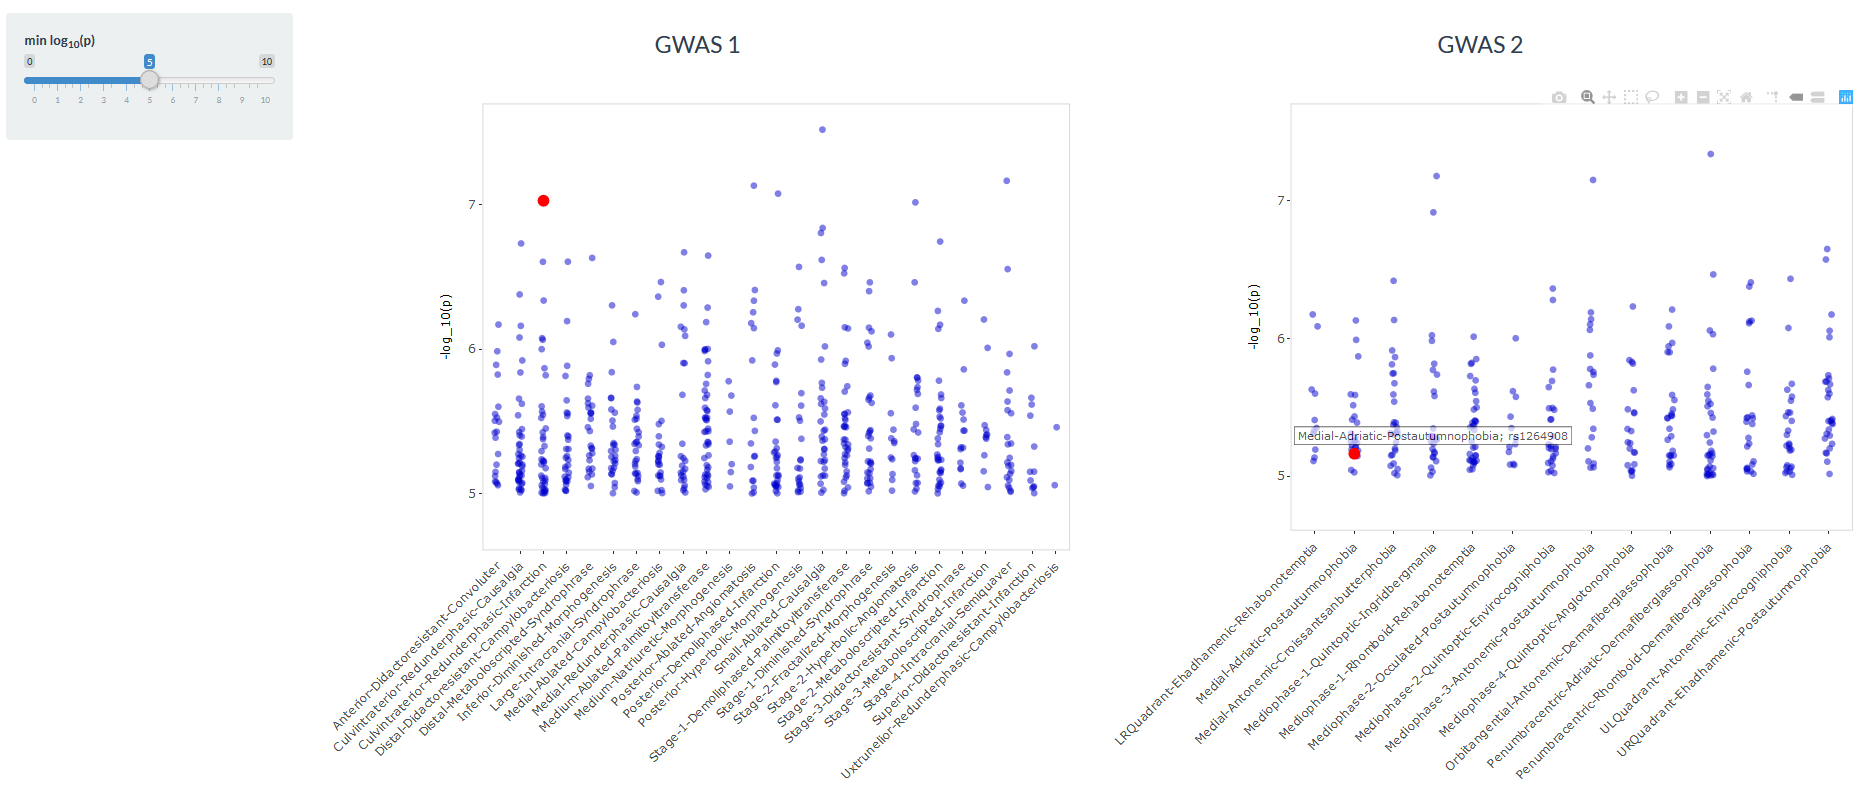
\includegraphics[width=6.5in, trim={0 0 0 0}, clip]{Tab1.png}
    \centering
    \caption{\texttt{plotly} pleiotropy app, tab 1, cross-GWAS phenotype SNP associations.}
    \label{fg:tab1}
\end{figure}


Important features (snnn indicates line number in \texttt{server.r}, fnnn indicates line number in the functions script):

\begin{itemize}
  \item (f38, f76) \texttt{ggplot} \texttt{geom\_jitter()} and \texttt{alpha} used to avoid point overlap
  \item (f54, f98) Axis text angle (explore themes here)
  \item (f38, f42, f77, f81) Hover labels automatically configured using \texttt{aes()} variables (note the inclusion of a user defined variable, SNP)
  \item (f41) Use of color to highlight selected points
  \item (s70-73) Annotation composition and assignment to plot 2 (labels for selected points)
  \item (f83, s71) Custom labels are added with \texttt{add\_annotations}, since \texttt{ggplotly()} does not convert them
  \item (s34, s65, s82) Use of \texttt{ggplotly()} to convert a \texttt{ggplot()} object to \texttt{plotly()}
  \item Point selection and control of events
  \begin{itemize}
      \item (s34) Plot 1 is rendered with source ID ``t1Plot1"
      \item (s43) A reactive event data object is created by the click event on a plot 1 point, with source ID ``t1Plot1"
      \item (s46-91) The selected plot 1 point (defined in the event data) is used to highlight associated points on plot 2
      \item (s77-82) The selected plot 1 point is highlighted (note the re-specification of source ID ``t1Plot1" recreating the reactive environment by source ID)
  \end{itemize}
  \item (s37, s82) Nested rendering of plots 
  \item (f76) Subsetting observations for selected point (\texttt{setdiff()})
  \item (f80-81) Coloring selected points using two geoms and data subsets in \texttt{t1ComposePlot2()}
\end{itemize}

%\clearpage
\vspace{0.25in}

Figure \ref{fg:tab2} is an example screen-shot of tab 2 of the pleiotropy app.  After filtering within-GWAS associations by significance (p), groups of inter-GWAS phenotypes are identified by clicking points in either set (left and right vertical blue dots).  Hovering over blue dots causes display of SNPs associated with a phenotype (within GWAS).  Hovering over a green dot (on an edge, or line connecting the GWAS sets) causes display of SNPs that are associated with the connected phenotypes (between GWAS). 

\begin{figure}[H]
    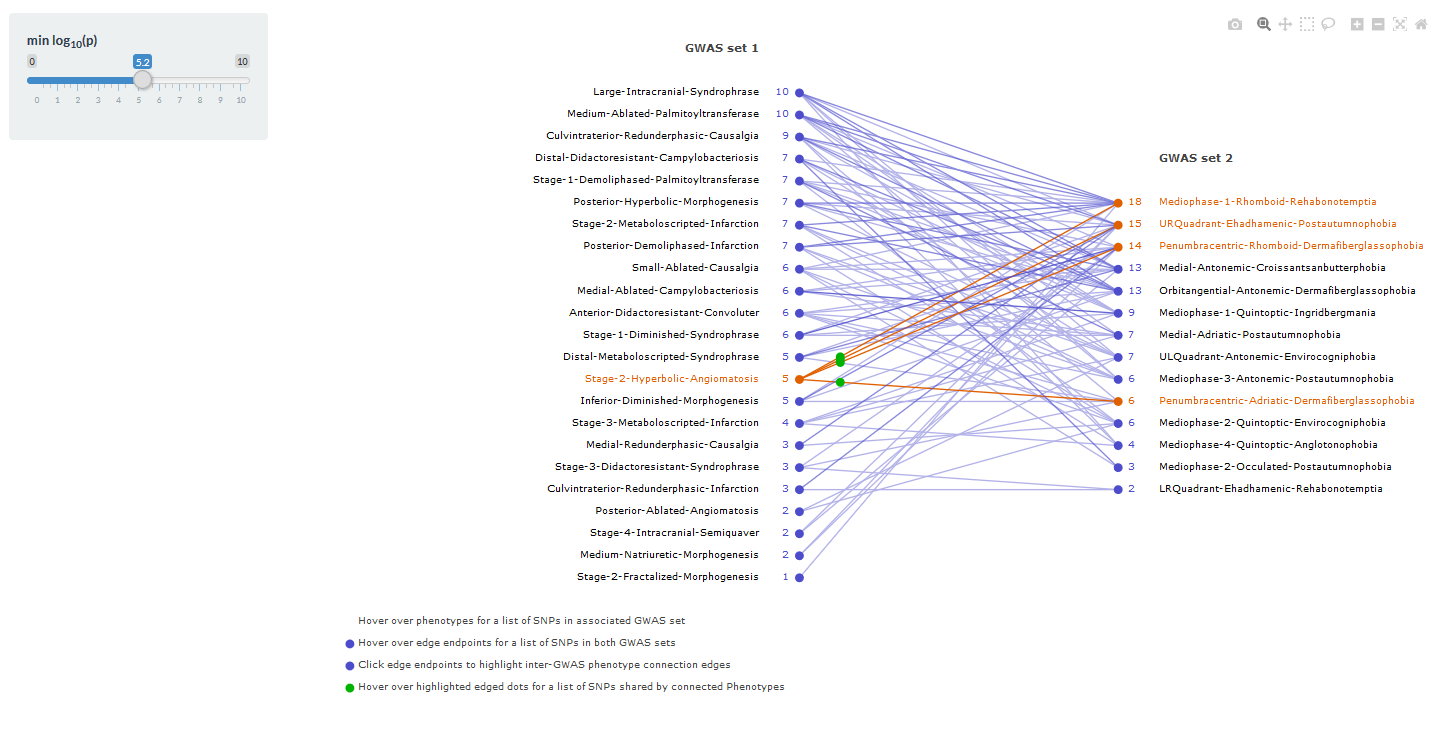
\includegraphics[width=6.5in, trim={0 0 0 0}, clip]{Tab2.png}
    \centering
    \caption{\texttt{plotly} pleiotropy app, tab 2, identification of phenotype association groups.  Associated SNPs appear as points are hovered over.}
    \label{fg:tab2}
\end{figure}

Important features:

\begin{itemize}
    \item Use of \texttt{plotly()} \%$>$\% to pipe output of one function into another
    \item Use of traces (similar to geoms) to display points, lines, and labels
    \begin{itemize}
        \item (f121-168) Phenotype labels
        \item (f237-247) Vertices (note the update of the graph object created during label trace addition)
        \item (f180-198) Edges connecting vertices
        \item (f203-232) Selected points
    \end{itemize}
    \item Subsetting plotted points by p-filter
    \item Phenotype ordering by number of associated SNPs
    \item Display of number of SNPs (\texttt{geom\_text()})
    \item Phenotype point hover labels
    \item Coloring vertices (phenotype) and edges (lines) of selected point (left and right)
    \item Display of green intersection point
    \item SNP intersection of lines, hover labels 
\end{itemize}

%%%%%%%%%%%%%%%%%%%%%%%%%%%%%%%%%%%%%%%%%%%%%%%%%%%%%%%%%%%%%%%%%%%%%%%%%%%%%%%%%%%%%%%%%%%%%%

\section{Debugging}\label{sec:debugging}

It is important that you have a means of communicating with your app during execution.  Unlike a typical R script, that can be executed one line at a time, with interactive review of variables, once a Shiny script launches, it executes without the console prompt.  Upon termination, some global variables may be available for examination, but you may not have reliable information on when they were last updated.  Error and warning messages are displayed in the console (and the terminal session when executed in a shell) and, fortunately, so are the results of \texttt{print()} and \texttt{cat()}.  When executed in RStudio, Shiny offers sophisticated debugger features (more info at \url{https://shiny.rstudio.com/articles/debugging.html}).  However, one of the simplest methods of communicating with your app during execution is to use \texttt{print()} (for a formatted or multi-element object, such as a data frame) or \texttt{cat(, file=stderr())} for ``small" objects.  \texttt{file=stderr()} causes displayed items to appear in red.  Output may also be written to an error log, depending on your OS.  Considerations include

\begin{itemize}
    \item Shiny reports line numbers in error messages relative to the related function (\texttt{ui()} or \texttt{server()}) and, although not always exact, reported lines are usually in the proximity of the one which was executed at the time of error
    \item \texttt{cat("your message here")} displays in RStudio console (generally, consider Shiny Server)
    \item \texttt{cat("your message here", file=stderr())} is treated as an error (red in console, logged by OS)
    \item Messages appear in RStudio console when Shiny app launched from within RStudio
    \item Messages appear in terminal window when Shiny app launched with the \texttt{rscript} command in shell
    \item There exists a ``showcase" mode (\texttt{runApp(display.mode="showcase")}) that is intended to highlight each line of your script as it is executing
    \item The reactivity log may be helpful in debugging reactive sequencing issues (\texttt{options(shiny.reactlog=T)}, \url{https://shiny.rstudio.com/reference/shiny/0.14/showReactLog.html}
    \url It may be helpful to initially format an app's appearance with an empty \texttt{server()} function, then include executable statements once the on-screen objects are available and configured
    \item Although not strictly related to debugging, the use of \texttt{gc()} to clear defunct memory (from R's recycling) may reduce total memory in use at a given time
\end{itemize}

\end{spacing}

\end{document} 